\documentclass{article}
\usepackage[T1]{fontenc}
\usepackage[utf8]{inputenc}
\usepackage{lmodern}
\usepackage[polish,shorthands=off]{babel}
\usepackage{graphicx}
\usepackage{siunitx}
\usepackage{multirow}
\usepackage{longtable}
\usepackage{hyperref}
\usepackage{float}
\title{Sprawozdanie obliczenia naukowe\\Lista 2}
\author{Jakub Kowal}
\date{}
\begin{document}
\maketitle

\section{Zadanie 1}
\subsection{Opis problemu}
Zadanie polega na wprowadzeniu niewielkich zmian do danych wejściowych, żeby sprawdzić uwaronkowanie zadania 5 z listy 1\\
\subsection{Wyniki}
Float64:\\
\\
\begin{tabular}{|c|c|c|}
    \hline
    Operacja & Typ & Wynik\\
    \hline
    \multirow{3}{*}{pa}&Stare Dane&\num{1.0251881368296672e-10}\\
    \cline{2-3}
    &Nowe Dane&\num{-0.004296342739891585}\\
    \cline{2-3}
    &Cond()&\num{4.19078478190021e7}\\
    \hline
    \multirow{3}{*}{pb}&Stare Dane&\num{-1.5643308870494366e-10}\\
    \cline{2-3}
    &Nowe Dane&\num{-0.004296342998713953}\\
    \cline{2-3}
    &Cond()&\num{2.7464412279069766e7}\\
    \hline
    \multirow{3}{*}{pc}&Stare Dane&\num{0.0}\\
    \cline{2-3}
    &Nowe Dane&\num{-0.004296342842280865}\\
    \cline{2-3}
    &Cond()&Inf\\
    \hline
    \multirow{3}{*}{pd}&Stare Dane&\num{0.0}\\
    \cline{2-3}
    &Nowe Dane&\num{-0.004296342842280865}\\
    \cline{2-3}
    &Cond()&Inf\\
    \hline
\end{tabular}\\\\
Float32:\\\\
\begin{tabular}{|c|c|c|}
    \hline
    Operacja & Typ & Wynik\\
    \hline
    \multirow{3}{*}{pa32}&Stare Dane&\num{-0.4999443}\\
    \cline{2-3}
    &Nowe Dane&\num{-0.4999443}\\
    \cline{2-3}
    &Cond()&\num{0.0}\\
    \hline
    \multirow{3}{*}{pb32}&Stare Dane&\num{-0.4543457}\\
    \cline{2-3}
    &Nowe Dane&\num{-0.4543457}\\
    \cline{2-3}
    &Cond()&\num{0.0}\\
    \hline
    \multirow{3}{*}{pc32}&Stare Dane&\num{-0.5}\\
    \cline{2-3}
    &Nowe Dane&\num{-0.5}\\
    \cline{2-3}
    &Cond()&\num{0.0}\\
    \hline
    \multirow{3}{*}{pd32}&Stare Dane&\num{-0.5}\\
    \cline{2-3}
    &Nowe Dane&\num{-0.5}\\
    \cline{2-3}
    &Cond()&\num{0.0}\\
    \hline
\end{tabular}\\
\subsection{Wnioski}
Dla Float64 zadanie jest bardzo źle uwarunkowane, ponieważ wskaźnik uwarunkowania zadania, jest bardzo duży. W przykładach c i d sięga nawet nieskończoności (przez dzielenie przez 0). Dla Float32 te zmiany nie wpływają na uwarunkowanie zadania, ponieważ nasze zmiany gubiły się podczas redukcji cyfr znaczących.\\

\section{Zadanie 2}
\subsection{Opis problemu}
W zadaniu trzeba narysować wykres funkcji:\\
\begin{center}
    $f(x)=e^{x}\ln(1+e^{-x})$
\end{center}
Następnie policzyć granicę:
\begin{center}
    $\lim_{x \to \infty}f(x)  $
\end{center}
Oraz porównać wykresy z wyliczoną granicą.
\subsection{Wyniki}
Granice:
\begin{center}
    $x\rightarrow -\infty$ lim = 0\\
    $x\rightarrow \infty$ lim = 1
\end{center}
\begin{figure}[H]
    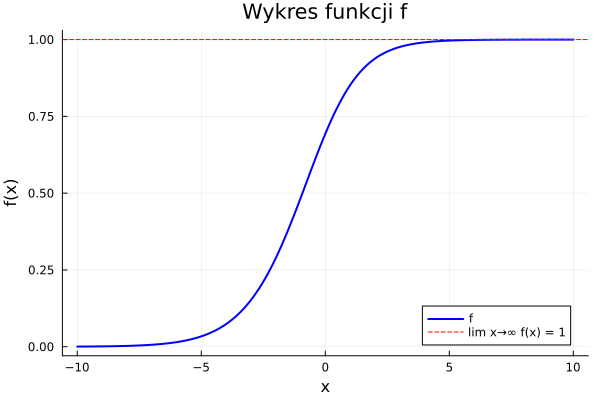
\includegraphics[width=120mm]{Z2_plot_julia.pdf}
    \caption{Wykres funkcji $f(x)$ wygenerowany w Julii}
    \label{fig:Z2_plot_julia}
\end{figure}
\begin{figure}[H]
    \includegraphics[width=120mm]{Z2_plot_py.png}
    \caption{Wykres funkcji $f(x)$ wygenerowany w pythonie}
    \label{fig:Z2_plot_python}
\end{figure}
\subsection{Wnioski}
Jak widać na wykresie \ref{fig:Z2_plot_julia} wygenerowanym w Julii, lub na wykresie \ref{fig:Z2_plot_python} wygenerowanym w pythonie, funkcja ta zbiega do $1$ zgodnie z wyliczoną granicą.

\section{Zadanie 3}
\subsection{Wyniki}
Wyniki dla Macierzy Hilb:\\
\begin{center}
    \begin{tabular}{|c|c|c|} 
    \hline
    N & Typ rozwiązania & Błąd względny \\
    \hline
    \multirow{2}{*}{1} & Gauss & \num{0.0} \\
    \cline{2-3}
    & Inv & \num{0.0} \\
    \hline
    \multirow{2}{*}{2} & Gauss & \num{5.661048867003676e-16} \\
    \cline{2-3}
    & Inv & \num{1.4043333874306803e-15} \\
    \hline
    \multirow{2}{*}{3} & Gauss & \num{8.022593772267726e-15} \\
    \cline{2-3}
    & Inv & \num{0.0} \\
    \hline
    \multirow{2}{*}{4} & Gauss & \num{4.137409622430382e-14} \\
    \cline{2-3}
    & Inv & \num{0.0} \\
    \hline
    \multirow{2}{*}{5} & Gauss & \num{1.6828426299227195e-12} \\
    \cline{2-3}
    & Inv & \num{3.3544360584359632e-12} \\
    \hline
    \multirow{2}{*}{6} & Gauss & \num{2.618913302311624e-10} \\
    \cline{2-3}
    & Inv & \num{2.0163759404347654e-10} \\
    \hline
    \multirow{2}{*}{7} & Gauss & \num{1.2606867224171548e-8} \\
    \cline{2-3}
    & Inv & \num{4.713280397232037e-9} \\
    \hline
    \multirow{2}{*}{8} & Gauss & \num{6.124089555723088e-8} \\
    \cline{2-3}
    & Inv & \num{3.07748390309622e-7} \\
    \hline
    \multirow{2}{*}{9} & Gauss & \num{3.8751634185032475e-6} \\
    \cline{2-3}
    & Inv & \num{4.541268303176643e-6} \\
    \hline
    \multirow{2}{*}{10} & Gauss & \num{8.67039023709691e-5} \\
    \cline{2-3}
    & Inv & \num{0.0002501493411824886} \\
    \hline
    \multirow{2}{*}{11} & Gauss & \num{0.00015827808158590435} \\
    \cline{2-3}
    & Inv & \num{0.007618304284315809} \\
    \hline
    \multirow{2}{*}{12} & Gauss & \num{0.13396208372085344} \\
    \cline{2-3}
    & Inv & \num{0.258994120804705} \\
    \hline
    \multirow{2}{*}{13} & Gauss & \num{0.11039701117868264} \\
    \cline{2-3}
    & Inv & \num{5.331275639426837} \\
    \hline
    \multirow{2}{*}{14} & Gauss & \num{1.4554087127659643} \\
    \cline{2-3}
    & Inv & \num{8.71499275104814} \\
    \hline
    \multirow{2}{*}{15} & Gauss & \num{4.696668350857427} \\
    \cline{2-3}
    & Inv & \num{7.344641453111494} \\
    \hline
    \multirow{2}{*}{16} & Gauss & \num{54.15518954564602} \\
    \cline{2-3}
    & Inv & \num{29.84884207073541} \\
    \hline
    \multirow{2}{*}{17} & Gauss & \num{13.707236683836307} \\
    \cline{2-3}
    & Inv & \num{10.516942378369349} \\
    \hline
    \multirow{2}{*}{18} & Gauss & \num{10.257619124632317} \\
    \cline{2-3}
    & Inv & \num{24.762070989128866} \\
    \hline
    \multirow{2}{*}{19} & Gauss & \num{102.15983486270827} \\
    \cline{2-3}
    & Inv & \num{109.94550732878284} \\
    \hline
    \multirow{2}{*}{20} & Gauss & \num{108.31777346206205} \\
    \cline{2-3}
    & Inv & \num{114.34403152557572} \\
    \hline
    \end{tabular}
\end{center}
Wyniki dla macierzy Matcond:\\
\begin{center}
    \begin{tabular}{|c|c|c|c|}
        \hline
        N & C & Typ rozwiązania & Błąd względny\\
        \hline
        \multirow{12}{*}{5} & \multirow{2}{*}{\num{1.0}} & Gauss & \num{2.220446049250313e-16}\\
        \cline{3-4}
        && Inv & \num{1.1102230246251565e-16}\\
        \cline{2-4}
        & \multirow{2}{*}{\num{10.0}} & Gauss & \num{7.818997388068909e-16}\\
        \cline{3-4}
        && Inv & \num{4.965068306494546e-16}\\
        \cline{2-4}
        & \multirow{2}{*}{\num{10000.0}} & Gauss & \num{1.4043333874306804e-16}\\
        \cline{3-4}
        && Inv & \num{1.3748588824509882e-13}\\
        \cline{2-4}
        & \multirow{2}{*}{\num{1.0e8}} & Gauss & \num{6.804459704896332e-10}\\
        \cline{3-4}
        && Inv & \num{6.333678266375997e-10}\\
        \cline{2-4}
        & \multirow{2}{*}{\num{1.0e13}} & Gauss & \num{0.00022935112010741482}\\
        \cline{3-4}
        && Inv & \num{8.631674575031098e-5}\\
        \cline{2-4}
        & \multirow{2}{*}{\num{1.0e17}} & Gauss & \num{3.188349061503315}\\
        \cline{3-4}
        && Inv & \num{0.4181840858850322}\\
        \hline
        \multirow{12}{*}{10} & \multirow{2}{*}{\num{1.0}} & Gauss & \num{1.7554167342883504e-16}\\
        \cline{3-4}
        && Inv & \num{2.937374022976103e-16}\\
        \cline{2-4}
        & \multirow{2}{*}{\num{10.0}} & Gauss & \num{4.168883761650163e-16}\\
        \cline{3-4}
        && Inv & \num{3.349121675321943e-16}\\
        \cline{2-4}
        & \multirow{2}{*}{\num{10000.0}} & Gauss & \num{1.986945058591428e-13}\\
        \cline{3-4}
        && Inv & \num{3.540793478199175e-14}\\
        \cline{2-4}
        & \multirow{2}{*}{\num{1.0e8}} & Gauss & \num{2.0215803771962333e-9}\\
        \cline{3-4}
        && Inv & \num{1.5391496830655643e-9}\\
        \cline{2-4}
        & \multirow{2}{*}{\num{1.0e13}} & Gauss & \num{0.00022366358147360663}\\
        \cline{3-4}
        && Inv & \num{0.00017290302092547966}\\
        \cline{2-4}
        & \multirow{2}{*}{\num{1.0e17}} & Gauss & \num{1.0881568942609348}\\
        \cline{3-4}
        && Inv & \num{0.22516448048909884}\\
        \hline
        \multirow{12}{*}{20} & \multirow{2}{*}{\num{1.0}} & Gauss & \num{5.484097192022683e-16}\\
        \cline{3-4}
        && Inv & \num{4.198346204284728e-16}\\
        \cline{2-4}
        & \multirow{2}{*}{\num{10.0}} & Gauss & \num{4.927689594407735e-16}\\
        \cline{3-4}
        && Inv & \num{5.376277206893598e-16}\\
        \cline{2-4}
        & \multirow{2}{*}{\num{10000.0}} & Gauss & \num{1.7823014177018397e-13}\\
        \cline{3-4}
        && Inv & \num{1.3158341555495355e-13}\\
        \cline{2-4}
        & \multirow{2}{*}{\num{1.0e8}} & Gauss & \num{4.606463401416786e-9}\\
        \cline{3-4}
        && Inv & \num{3.9804209926076523e-10}\\
        \cline{2-4}
        & \multirow{2}{*}{\num{1.0e13}} & Gauss & \num{4.3760807738426575e-5}\\
        \cline{3-4}
        && Inv & \num{1.3787109656144105e-5}\\
        \cline{2-4}
        & \multirow{2}{*}{\num{1.0e17}} & Gauss & \num{3.0894724052108167}\\
        \cline{3-4}
        && Inv & \num{0.2542425657252587}\\
        \hline
    \end{tabular}
\end{center}
Wyniki cond dla macierzy rzędu 6 (oraz c = $10^{7}$)\\
Cond A hilb: $1.4951058642254665*10^{7}$\\
Cond A matcond: $1.000000003815985*10^{8}$\\
\subsection{Wnioski}
Błędy względne tych dwóch algorytmów są bardzo zbliżone, ale wydaje mi się, że algorytm z inwersją osiągał niższe błędy. Ponadto macierz matcond podczas obliczeń wykazywała o wiele mniejsze błędy względne.\\

\section{Zadanie 4}
\subsection{Opis problemu}
Mamy obliczyć miejsca zerowe wielomianu funkcją $roots()$, następnie porównać obliczone miejsca zerowe do prawdziwych (liczby od 1 do 20). Dodatkowo spróbować obliczyć te wielomiany za pomocą miejsc zerowych oraz wyjaśnić skąd się biorą rozbieżności. Powtórzyć eksperyment dla zaburzonych danych oraz wyjaśnić zjawisko.
\subsection{Wyniki}
\subsubsection*{A)}
\begin{center}
    \begin{longtable}{|c|c|c|}
        \caption*{Tabela bez zmian współczynnika}
    \label{tab:table1}\\
    \hline
    Obliczone miejsce zerowe & Operacja & Wynik \\
    \hline
    \endfirsthead
    \hline
    Obliczone miejsce zerowe & Operacja & Wynik \\
    \hline
    \endhead
    \multirow{3}{*}{0.9999999999996989} & $|P(Z_k)|$ & \num{35696.50964788257} \\
    \cline{2-3}
    & $|p(Z_k)|$ & \num{36626.425482422805} \\
    \cline{2-3}
    & $|k - z_k|$ & \num{3.0109248427834245e-13} \\
    \hline
    \multirow{3}{*}{2.0000000000283182} & $|P(Z_k)|$ & \num{176252.60026668405} \\
    \cline{2-3}
    & $|p(Z_k)|$ & \num{181303.93367257662} \\
    \cline{2-3}
    & $|k - z_k|$ & \num{2.8318236644508943e-11} \\
    \hline
    \multirow{3}{*}{2.9999999995920965} & $|P(Z_k)|$ & \num{279157.6968824087} \\
    \cline{2-3}
    & $|p(Z_k)|$ & \num{290172.2858891686} \\
    \cline{2-3}
    & $|k - z_k|$ & \num{4.0790348876384996e-10} \\
    \hline
    \multirow{3}{*}{3.9999999837375317} & $|P(Z_k)|$ & \num{3.0271092988991085e6} \\
    \cline{2-3}
    & $|p(Z_k)|$ & \num{2.0415372902750901e6} \\
    \cline{2-3}
    & $|k - z_k|$ & \num{1.626246826091915e-8} \\
    \hline
    \multirow{3}{*}{5.000000665769791} & $|P(Z_k)|$ & \num{2.2917473756567076e7} \\
    \cline{2-3}
    & $|p(Z_k)|$ & \num{2.0894625006962188e7} \\
    \cline{2-3}
    & $|k - z_k|$ & \num{6.657697912970661e-7} \\
    \hline
    \multirow{3}{*}{5.999989245824773} & $|P(Z_k)|$ & \num{1.2902417284205095e8} \\
    \cline{2-3}
    & $|p(Z_k)|$ & \num{1.1250484577562995e8} \\
    \cline{2-3}
    & $|k - z_k|$ & \num{1.0754175226779239e-5} \\
    \hline
    \multirow{3}{*}{7.000102002793008} & $|P(Z_k)|$ & \num{4.805112754602064e8} \\
    \cline{2-3}
    & $|p(Z_k)|$ & \num{4.572908642730946e8} \\
    \cline{2-3}
    & $|k - z_k|$ & \num{0.00010200279300764947} \\
    \hline
    \multirow{3}{*}{7.999355829607762} & $|P(Z_k)|$ & \num{1.6379520218961136e9} \\
    \cline{2-3}
    & $|p(Z_k)|$ & \num{1.5556459377357383e9} \\
    \cline{2-3}
    & $|k - z_k|$ & \num{0.0006441703922384079} \\
    \hline
    \multirow{3}{*}{9.002915294362053} & $|P(Z_k)|$ & \num{4.877071372550003e9} \\
    \cline{2-3}
    & $|p(Z_k)|$ & \num{4.687816175648389e9} \\
    \cline{2-3}
    & $|k - z_k|$ & \num{0.002915294362052734} \\
    \hline
    \multirow{3}{*}{9.990413042481725} & $|P(Z_k)|$ & \num{1.3638638195458128e10} \\
    \cline{2-3}
    & $|p(Z_k)|$ & \num{1.2634601896949205e10} \\
    \cline{2-3}
    & $|k - z_k|$ & \num{0.009586957518274986} \\
    \hline
    \multirow{3}{*}{11.025022932909318} & $|P(Z_k)|$ & \num{3.585631295130865e10} \\
    \cline{2-3}
    & $|p(Z_k)|$ & \num{3.300128474498415e10} \\
    \cline{2-3}
    & $|k - z_k|$ & \num{0.025022932909317674} \\
    \hline
    \multirow{3}{*}{11.953283253846857} & $|P(Z_k)|$ & \num{7.533332360358197e10} \\
    \cline{2-3}
    & $|p(Z_k)|$ & \num{7.388525665404988e10} \\
    \cline{2-3}
    & $|k - z_k|$ & \num{0.04671674615314281} \\
    \hline
    \multirow{3}{*}{13.07431403244734} & $|P(Z_k)|$ & \num{1.9605988124330817e11} \\
    \cline{2-3}
    & $|p(Z_k)|$ & \num{1.8476215093144193e11} \\
    \cline{2-3}
    & $|k - z_k|$ & \num{0.07431403244734014} \\
    \hline
    \multirow{3}{*}{13.914755591802127} & $|P(Z_k)|$ & \num{3.5751347823104315e11} \\
    \cline{2-3}
    & $|p(Z_k)|$ & \num{3.5514277528420844e11} \\
    \cline{2-3}
    & $|k - z_k|$ & \num{0.08524440819787316} \\
    \hline
    \multirow{3}{*}{15.075493799699476} & $|P(Z_k)|$ & \num{8.21627123645597e11} \\
    \cline{2-3}
    & $|p(Z_k)|$ & \num{8.423201558964254e11} \\
    \cline{2-3}
    & $|k - z_k|$ & \num{0.07549379969947623} \\
    \hline
    \multirow{3}{*}{15.946286716607972} & $|P(Z_k)|$ & \num{1.5514978880494067e12} \\
    \cline{2-3}
    & $|p(Z_k)|$ & \num{1.570728736625802e12} \\
    \cline{2-3}
    & $|k - z_k|$ & \num{0.05371328339202819} \\
    \hline
    \multirow{3}{*}{17.025427146237412} & $|P(Z_k)|$ & \num{3.694735918486229e12} \\
    \cline{2-3}
    & $|p(Z_k)|$ & \num{3.3169782238892363e12} \\
    \cline{2-3}
    & $|k - z_k|$ & \num{0.025427146237412046} \\
    \hline
    \multirow{3}{*}{17.99092135271648} & $|P(Z_k)|$ & \num{7.650109016515867e12} \\
    \cline{2-3}
    & $|p(Z_k)|$ & \num{6.34485314179128e12} \\
    \cline{2-3}
    & $|k - z_k|$ & \num{0.009078647283519814} \\
    \hline
    \multirow{3}{*}{19.00190981829944} & $|P(Z_k)|$ & \num{1.1435273749721195e13} \\
    \cline{2-3}
    & $|p(Z_k)|$ & \num{1.228571736671966e13} \\
    \cline{2-3}
    & $|k - z_k|$ & \num{0.0019098182994383706} \\
    \hline
    \multirow{3}{*}{19.999809291236637} & $|P(Z_k)|$ & \num{2.7924106393680727e13} \\
    \cline{2-3}
    & $|p(Z_k)|$ & \num{2.318309535271638e13} \\
    \cline{2-3}
    & $|k - z_k|$ & \num{0.00019070876336257925} \\
    \hline
    \end{longtable}
\end{center}

    \subsubsection*{B) }

    \begin{center}
    \begin{longtable}{|c|c|c|}
        \caption*{Tabela ze zmianą współczynnika}
        \label{tab:table2}\\
    \hline
    Obliczone miejsce zerowe & Operacja & Wynik \\
    \hline
    \endfirsthead 
    \hline
    Obliczone miejsce zerowe & Operacja & Wynik \\
    \hline
    \endhead
        \multirow{3}{*}{0.9999999999998357 + 0.0im} & $|P(Z_k)|$ & \num{20259.872313418207} \\
        \cline{2-3}
        & $|p(Z_k)|$ & \num{19987.872313406835} \\
        \cline{2-3}
        & $|k - z_k|$ & \num{1.6431300764452317e-13} \\
        \hline
        \multirow{3}{*}{2.0000000000550373 + 0.0im} & $|P(Z_k)|$ & \num{346541.4137593836} \\
        \cline{2-3}
        & $|p(Z_k)|$ & \num{352369.4138087958} \\
        \cline{2-3}
        & $|k - z_k|$ & \num{5.503730804434781e-11} \\
        \hline
        \multirow{3}{*}{2.99999999660342 + 0.0im} & $|P(Z_k)|$ & \num{2.2580597001197007e6} \\
        \cline{2-3}
        & $|p(Z_k)|$ & \num{2.4162415582518433e6} \\
        \cline{2-3}
        & $|k - z_k|$ & \num{3.3965799062229962e-9} \\
        \hline
        \multirow{3}{*}{4.000000089724362 + 0.0im} & $|P(Z_k)|$ & \num{1.0542631790395478e7} \\
        \cline{2-3}
        & $|p(Z_k)|$ & \num{1.1263702300292023e7} \\
        \cline{2-3}
        & $|k - z_k|$ & \num{8.972436216225788e-8} \\
        \hline
        \multirow{3}{*}{4.99999857388791 + 0.0im} & $|P(Z_k)|$ & \num{3.757830916585153e7} \\
        \cline{2-3}
        & $|p(Z_k)|$ & \num{4.475744423806908e7} \\
        \cline{2-3}
        & $|k - z_k|$ & \num{1.4261120897529622e-6} \\
        \hline
        \multirow{3}{*}{6.000020476673031 + 0.0im} & $|P(Z_k)|$ & \num{1.3140943325569446e8} \\
        \cline{2-3}
        & $|p(Z_k)|$ & \num{2.1421031658039317e8} \\
        \cline{2-3}
        & $|k - z_k|$ & \num{2.0476673030955794e-5} \\
        \hline
        \multirow{3}{*}{6.99960207042242 + 0.0im} & $|P(Z_k)|$ & \num{3.939355874647618e8} \\
        \cline{2-3}
        & $|p(Z_k)|$ & \num{1.7846173427860644e9} \\
        \cline{2-3}
        & $|k - z_k|$ & \num{0.00039792957757978087} \\
        \hline
        \multirow{3}{*}{8.007772029099446 + 0.0im} & $|P(Z_k)|$ & \num{1.184986961371896e9} \\
        \cline{2-3}
        & $|p(Z_k)|$ & \num{1.8686972170009857e10} \\
        \cline{2-3}
        & $|k - z_k|$ & \num{0.007772029099445632} \\
        \hline
        \multirow{3}{*}{8.915816367932559 + 0.0im} & $|P(Z_k)|$ & \num{2.2255221233077707e9} \\
        \cline{2-3}
        & $|p(Z_k)|$ & \num{1.3746309775142993e11} \\
        \cline{2-3}
        & $|k - z_k|$ & \num{0.0841836320674414} \\
        \hline
        \multirow{3}{*}{10.095455630535774 - 0.6449328236240688im} & $|P(Z_k)|$ & \num{1.0677921232930157e10} \\
        \cline{2-3}
        & $|p(Z_k)|$ & \num{1.490069535200058e12} \\
        \cline{2-3}
        & $|k - z_k|$ & \num{0.6519586830380407} \\
        \hline
        \multirow{3}{*}{10.095455630535774 + 0.6449328236240688im} & $|P(Z_k)|$ & \num{1.0677921232930157e10} \\
        \cline{2-3}
        & $|p(Z_k)|$ & \num{1.490069535200058e12} \\
        \cline{2-3}
        & $|k - z_k|$ & \num{1.1109180272716561} \\
        \hline
        \multirow{3}{*}{11.793890586174369 - 1.6524771364075785im} & $|P(Z_k)|$ & \num{3.1401962344429485e10} \\
        \cline{2-3}
        & $|p(Z_k)|$ & \num{3.2962792355717145e13} \\
        \cline{2-3}
        & $|k - z_k|$ & \num{1.665281290598479} \\
        \hline
        \multirow{3}{*}{11.793890586174369 + 1.6524771364075785im} & $|P(Z_k)|$ & \num{3.1401962344429485e10} \\
        \cline{2-3}
        & $|p(Z_k)|$ & \num{3.2962792355717145e13} \\
        \cline{2-3}
        & $|k - z_k|$ & \num{2.0458202766784277} \\
        \hline
        \multirow{3}{*}{13.992406684487216 - 2.5188244257108443im} & $|P(Z_k)|$ & \num{2.157665405951858e11} \\
        \cline{2-3}
        & $|p(Z_k)|$ & \num{9.546022365750216e14} \\
        \cline{2-3}
        & $|k - z_k|$ & \num{2.518835871190904} \\
        \hline
        \multirow{3}{*}{13.992406684487216 + 2.5188244257108443im} & $|P(Z_k)|$ & \num{2.157665405951858e11} \\
        \cline{2-3}
        & $|p(Z_k)|$ & \num{9.546022365750216e14} \\
        \cline{2-3}
        & $|k - z_k|$ & \num{2.7128805312847097} \\
        \hline
        \multirow{3}{*}{16.73074487979267 - 2.812624896721978im} & $|P(Z_k)|$ & \num{4.850110893921027e11} \\
        \cline{2-3}
        & $|p(Z_k)|$ & \num{2.742106076928478e16} \\
        \cline{2-3}
        & $|k - z_k|$ & \num{2.9060018735375106} \\
        \hline
        \multirow{3}{*}{16.73074487979267 + 2.812624896721978im} & $|P(Z_k)|$ & \num{4.850110893921027e11} \\
        \cline{2-3}
        & $|p(Z_k)|$ & \num{2.742106076928478e16} \\
        \cline{2-3}
        & $|k - z_k|$ & \num{2.825483521349608} \\
        \hline
        \multirow{3}{*}{19.5024423688181 - 1.940331978642903im} & $|P(Z_k)|$ & \num{4.557199223869993e12} \\
        \cline{2-3}
        & $|p(Z_k)|$ & \num{4.2524858765203725e17} \\
        \cline{2-3}
        & $|k - z_k|$ & \num{2.4540214463129764} \\
        \hline
        \multirow{3}{*}{19.5024423688181 + 1.940331978642903im} & $|P(Z_k)|$ & \num{4.557199223869993e12} \\
        \cline{2-3}
        & $|p(Z_k)|$ & \num{4.2524858765203725e17} \\
        \cline{2-3}
        & $|k - z_k|$ & \num{2.0043294443099486} \\
        \hline
        \multirow{3}{*}{20.84691021519479 + 0.0im} & $|P(Z_k)|$ & \num{8.756386551865696e12} \\
        \cline{2-3}
        & $|p(Z_k)|$ & \num{1.37437435599976e18} \\
        \cline{2-3}
        & $|k - z_k|$ & \num{0.8469102151947894} \\
        \hline
    \end{longtable}
     \end{center}

\subsection{Wnioski}
Proces jest niestabilny, bo widać że niewielkie zmiany w danych nakładają się i kumulują w większe dysproporcje. Dodatkowo zauważamy jak zaokrąglanie liczb powoduje niepoprawne wyniki przy obliczaniu wyników wielomianów. W tabelach \ref{tab:table1} i \ref{tab:table2} jasno ukazuje się wielka dysproporcja w wynikach (które powinny być równe 0). Wielomian Wilkinsona jest źle uwarunkowany, ponieważ delikatne zmiany w danych prowadzą do dużych zmian w wyniku. Ponadto poprzez zaburzenie jednego współczynnika o liczbę $\epsilon$ powoduje wielkie zmiany w miejscach zerowych wyliczanych przez $roots()$. Pojawiają się "zera zespolone" oraz miejsca zerowe się powtarzają z innym znakiem przy części urojonej. Dlaczego dochodzi do tak dużych błędów? Te minimalne zmiany w połączeniu z obrzymimi liczbami powodują redukcję cyfr znaczących, co prowadzi do kolejnych błędnych zaokrągleń i redukcji.

\section{Zadanie 5}
\subsection{Opis problemu}
Rozważamy równanie:
\begin{center}
    $p_{n+1} = p_{n} + rp_{n}(1-p_{n})$
\end{center}
dla danych $p_{0} = 0,01$ i $r = 3$. Mamy wykonać 40 iteracji oraz 40 iteracji z obcięciem liczby po 10 iteracji w arytmetyce Float32. Ponadto wykonać 40 iteracji tego równania w arytmetyce Float64 i porównać wyniki.
\subsection{Wyniki}
\begin{figure}[H]
    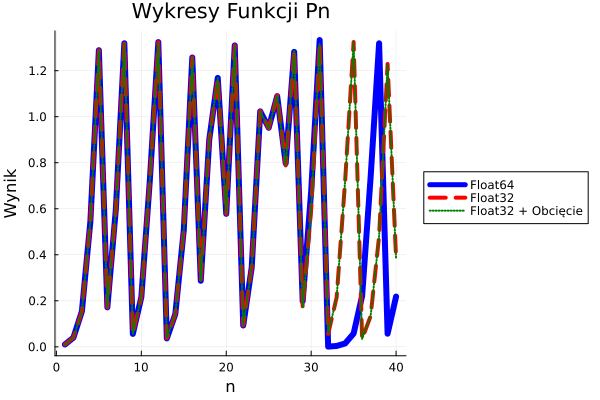
\includegraphics[width=120mm]{Z5_plot.pdf}
    \caption{Wyniki równań zadania 5}
    \label{fig:Z5}
\end{figure}
\subsection{Wnioski}
Wykres wyników zadania piątego \ref{fig:Z5} idealnie obrazuje nam zjawisko niestabilności. Porównując wykresy funkcji dla Float32 możemy zauważyć jak błędy wynikające z obcięcia cyfr rosną znacząco razem z kolejnymi iteracjami. Błędy zaczynają się od niewielkich różnic, ale wraz z kolejnymi iteracjami znacząco odbiegają od poprawnego wyniku. Wyniki dla Float64 odbiegają od tych dla Float32, co oznacza, że zaokrąglenia też powodują tutaj niestabilność. Mają one wpływ na kolejne iteracje co kumuluje błędy.

\section{Zadanie 6}
\subsection{Opis zadania}
Rozważamy równanie:
\begin{center}
    $x_{n+1} = x^{2}_{n}+c$
\end{center}
dla różnych danych $c$ i $x_{0}$. Mamy zwrócić uwagę na zachowanie tych ciągów.
\subsection{Wyniki}
\begin{figure}[H]
    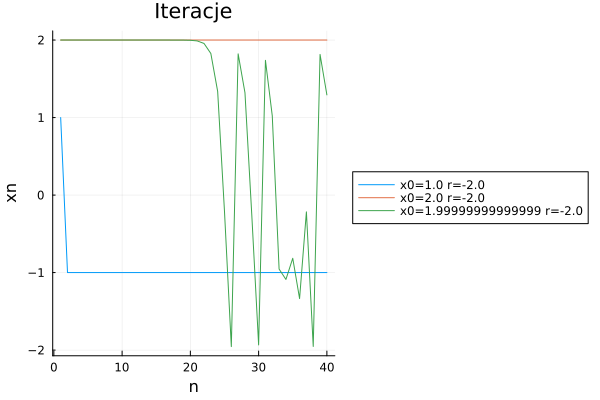
\includegraphics[width=120mm]{Z6_plot_v1.pdf}
    \caption{Wyniki dla 1), 2), 3)}
    \label{fig:Z6_1}
\end{figure}
\begin{figure}[H]
    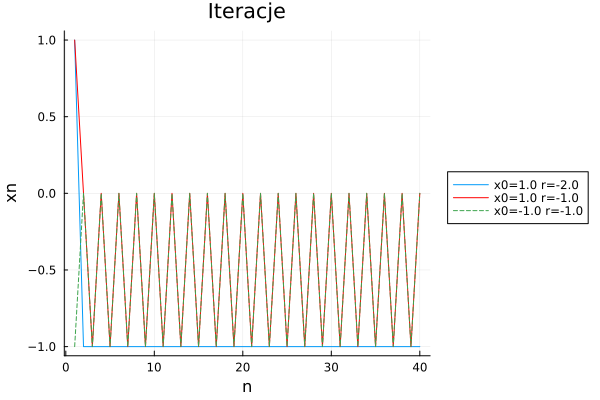
\includegraphics[width=120mm]{Z6_plot_v2.pdf}
    \caption{Wyniki dla 1), 4), 5)}
    \label{fig:Z6_2}
\end{figure}
\begin{figure}[H]
    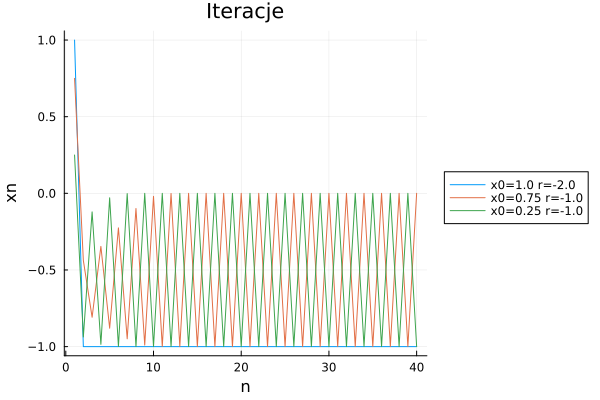
\includegraphics[width=120mm]{Z6_plot_v3.pdf}
    \caption{Wyniki dla 1), 6), 7)}
    \label{fig:Z6_3}
\end{figure}
\begin{figure}[H]
    \includegraphics[width=120mm]{Z6_spider_1.png}
    \caption{Wykres pajęczynowy dla 1)}
    \label{fig:Z6_s_1}
\end{figure}
\begin{figure}[H]
    \includegraphics[width=120mm]{Z6_spider_2.png}
    \caption{Wykres pajęczynowy dla 2)}
    \label{fig:Z6_s_2}
\end{figure}
\begin{figure}[H]
    \includegraphics[width=120mm]{Z6_spider_3.png}
    \caption{Wykres pajęczynowy dla 3)\\ Julia sama zaokrągliła x0 do 2.0}
    \label{fig:Z6_s_3}
\end{figure}
\begin{figure}[H]
    \includegraphics[width=120mm]{Z6_spider_4.png}
    \caption{Wykres pajęczynowy dla 4)}
    \label{fig:Z6_s_4}
\end{figure}
\begin{figure}[H]
    \includegraphics[width=120mm]{Z6_spider_5.png}
    \caption{Wykres pajęczynowy dla 5)}
    \label{fig:Z6_s_5}
\end{figure}
\begin{figure}[H]
    \includegraphics[width=120mm]{Z6_spider_6.png}
    \caption{Wykres pajęczynowy dla 6)}
    \label{fig:Z6_s_6}
\end{figure}
\begin{figure}[H]
    \includegraphics[width=120mm]{Z6_spider_7.png}
    \caption{Wykres pajęczynowy dla 7)}
    \label{fig:Z6_s_7}
\end{figure}
\subsection{Wnioski}
Na wykresach i diagramach pajęczynowych można zauważyć, że to równanie rekurencyjne zmierza do powtarzających się liczb, najczęściej 0 oraz -1. Wyjątkiem od tych powtarzających się wyników jest \ref{fig:Z6_s_3}, gdzie zaburzenie danych względem \ref{fig:Z6_s_2} powoduje błędy, które nie wykazują żadnej powtarzalności.\\


\section*{Adnotacje}
Wykresy pajęczynowe i wykres do zadania 2 stworzony w pythonie zostały stworzone przez sztuczną inteligencję.
\end{document}